\chapter{Architecture fonctionnelle cible du Smart WMS}
\section{Principes de conception}
L'architecture cible est construite comme un système modulaire. Elle doit pouvoir s'appliquer à un entrepôt simple utilisant des terminaux RF, mais aussi à un site automatisé intégrant RFID, convoyeurs, AMR/AGV, WCS/WES ou BMS/EMS. Le modèle distingue donc les blocs fonctionnels stables, les services Smart activables par la donnée et les options dépendantes de l'infrastructure.

\section{Vue d'ensemble}
La figure~\ref{fig:architecture-fonctionnelle} redessine la vue fonctionnelle cible à partir de l'architecture validée dans le support de benchmark. Contrairement à une représentation trop compacte, elle sépare explicitement les systèmes externes, le cœur opérationnel, la gestion des tâches, les données de référence, le stockage des données, les ressources et infrastructures, l'intelligence décisionnelle et les appareils terrain.

\begin{landscape}
\begin{figure}[p]
\centering
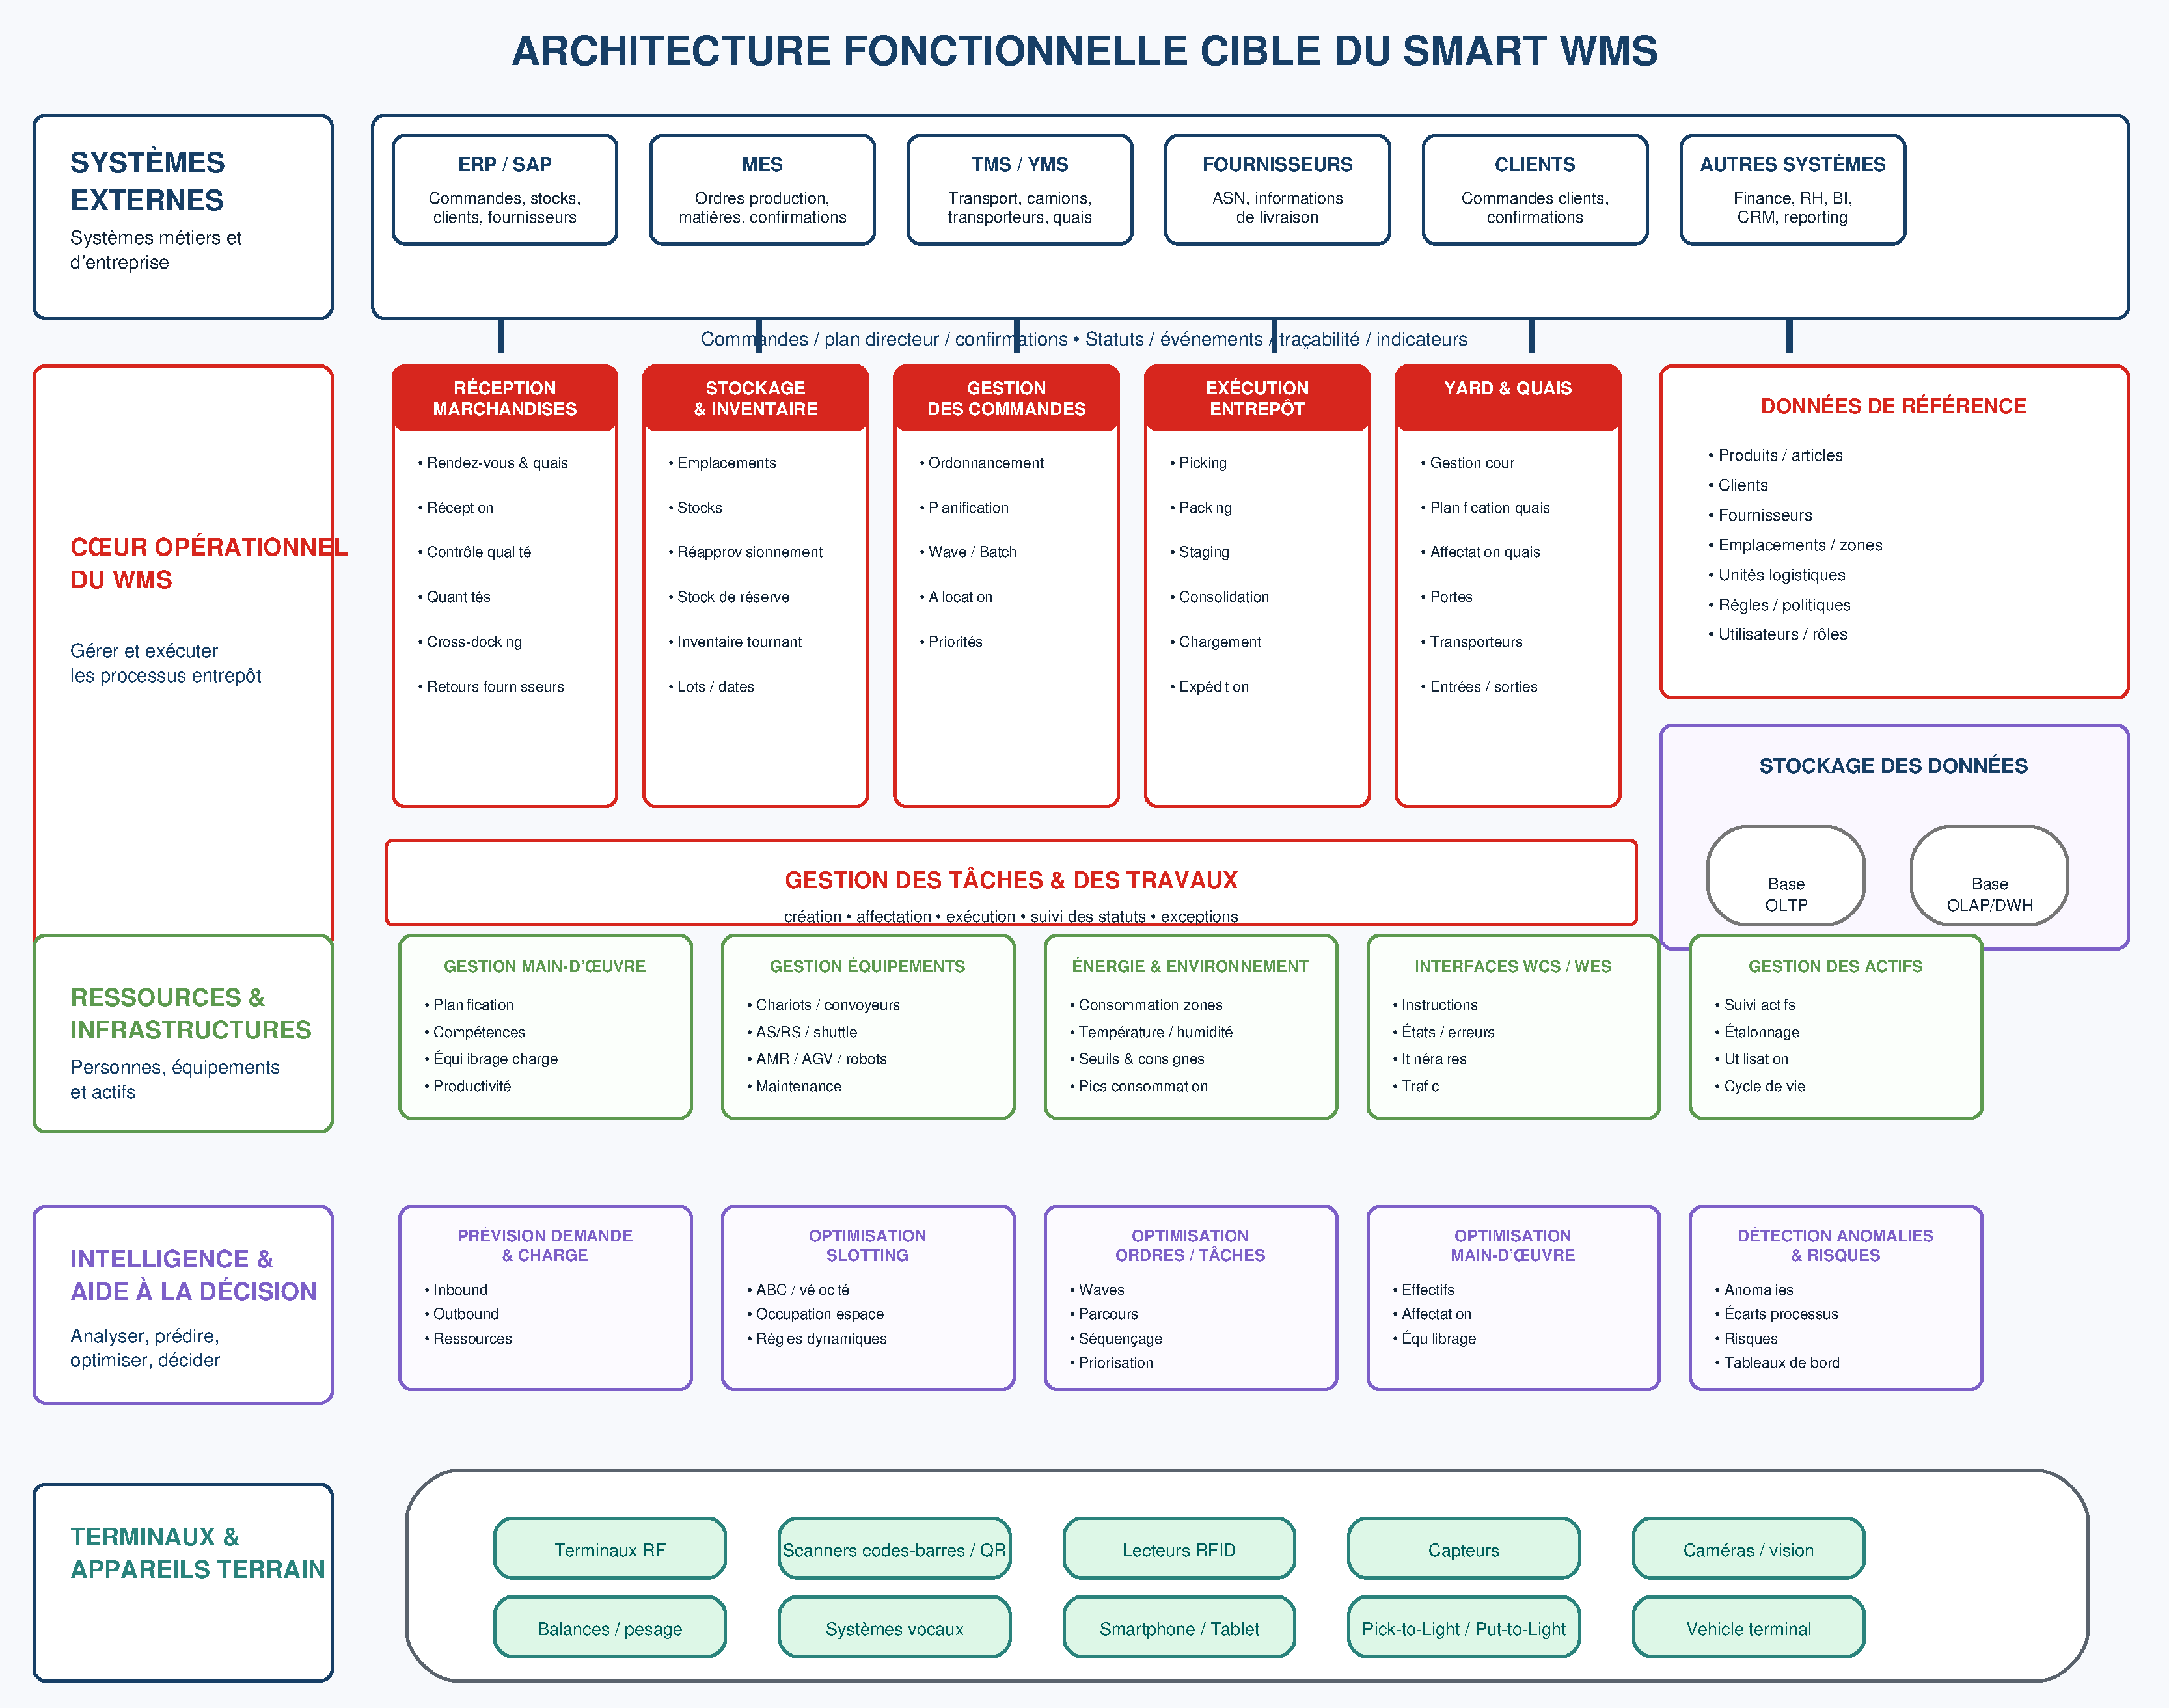
\includegraphics[width=0.98\linewidth]{figures/chapitre4/architecture_fonctionnelle.pdf}
\caption{Architecture fonctionnelle cible du Smart WMS proposée.}
\label{fig:architecture-fonctionnelle}
\end{figure}
\end{landscape}

\section{Rôle des couches}
Les systèmes externes alimentent le WMS en commandes, statuts, confirmations, informations transport, production et référentiels. Le cœur opérationnel exécute les processus d'entrepôt : réception, stockage, inventaire, commandes, préparation, expédition et yard. La gestion des tâches transforme les décisions en actions exécutables et assure le suivi des statuts et exceptions.

Les données de référence ne sont pas traitées comme des use cases artificiels. Elles constituent une couche de support essentielle : produits, clients, fournisseurs, zones, règles, unités logistiques, utilisateurs et rôles. Le stockage est séparé en deux usages : l'OLTP pour l'exécution transactionnelle et l'OLAP/DWH pour l'historique, les KPI, l'analyse et les modèles prédictifs.

\section{Activation progressive}
L'architecture doit rester utile même lorsque toutes les technologies ne sont pas disponibles. La figure~\ref{fig:activation-progressive} formalise cette progressivité.

\begin{figure}[H]
\centering
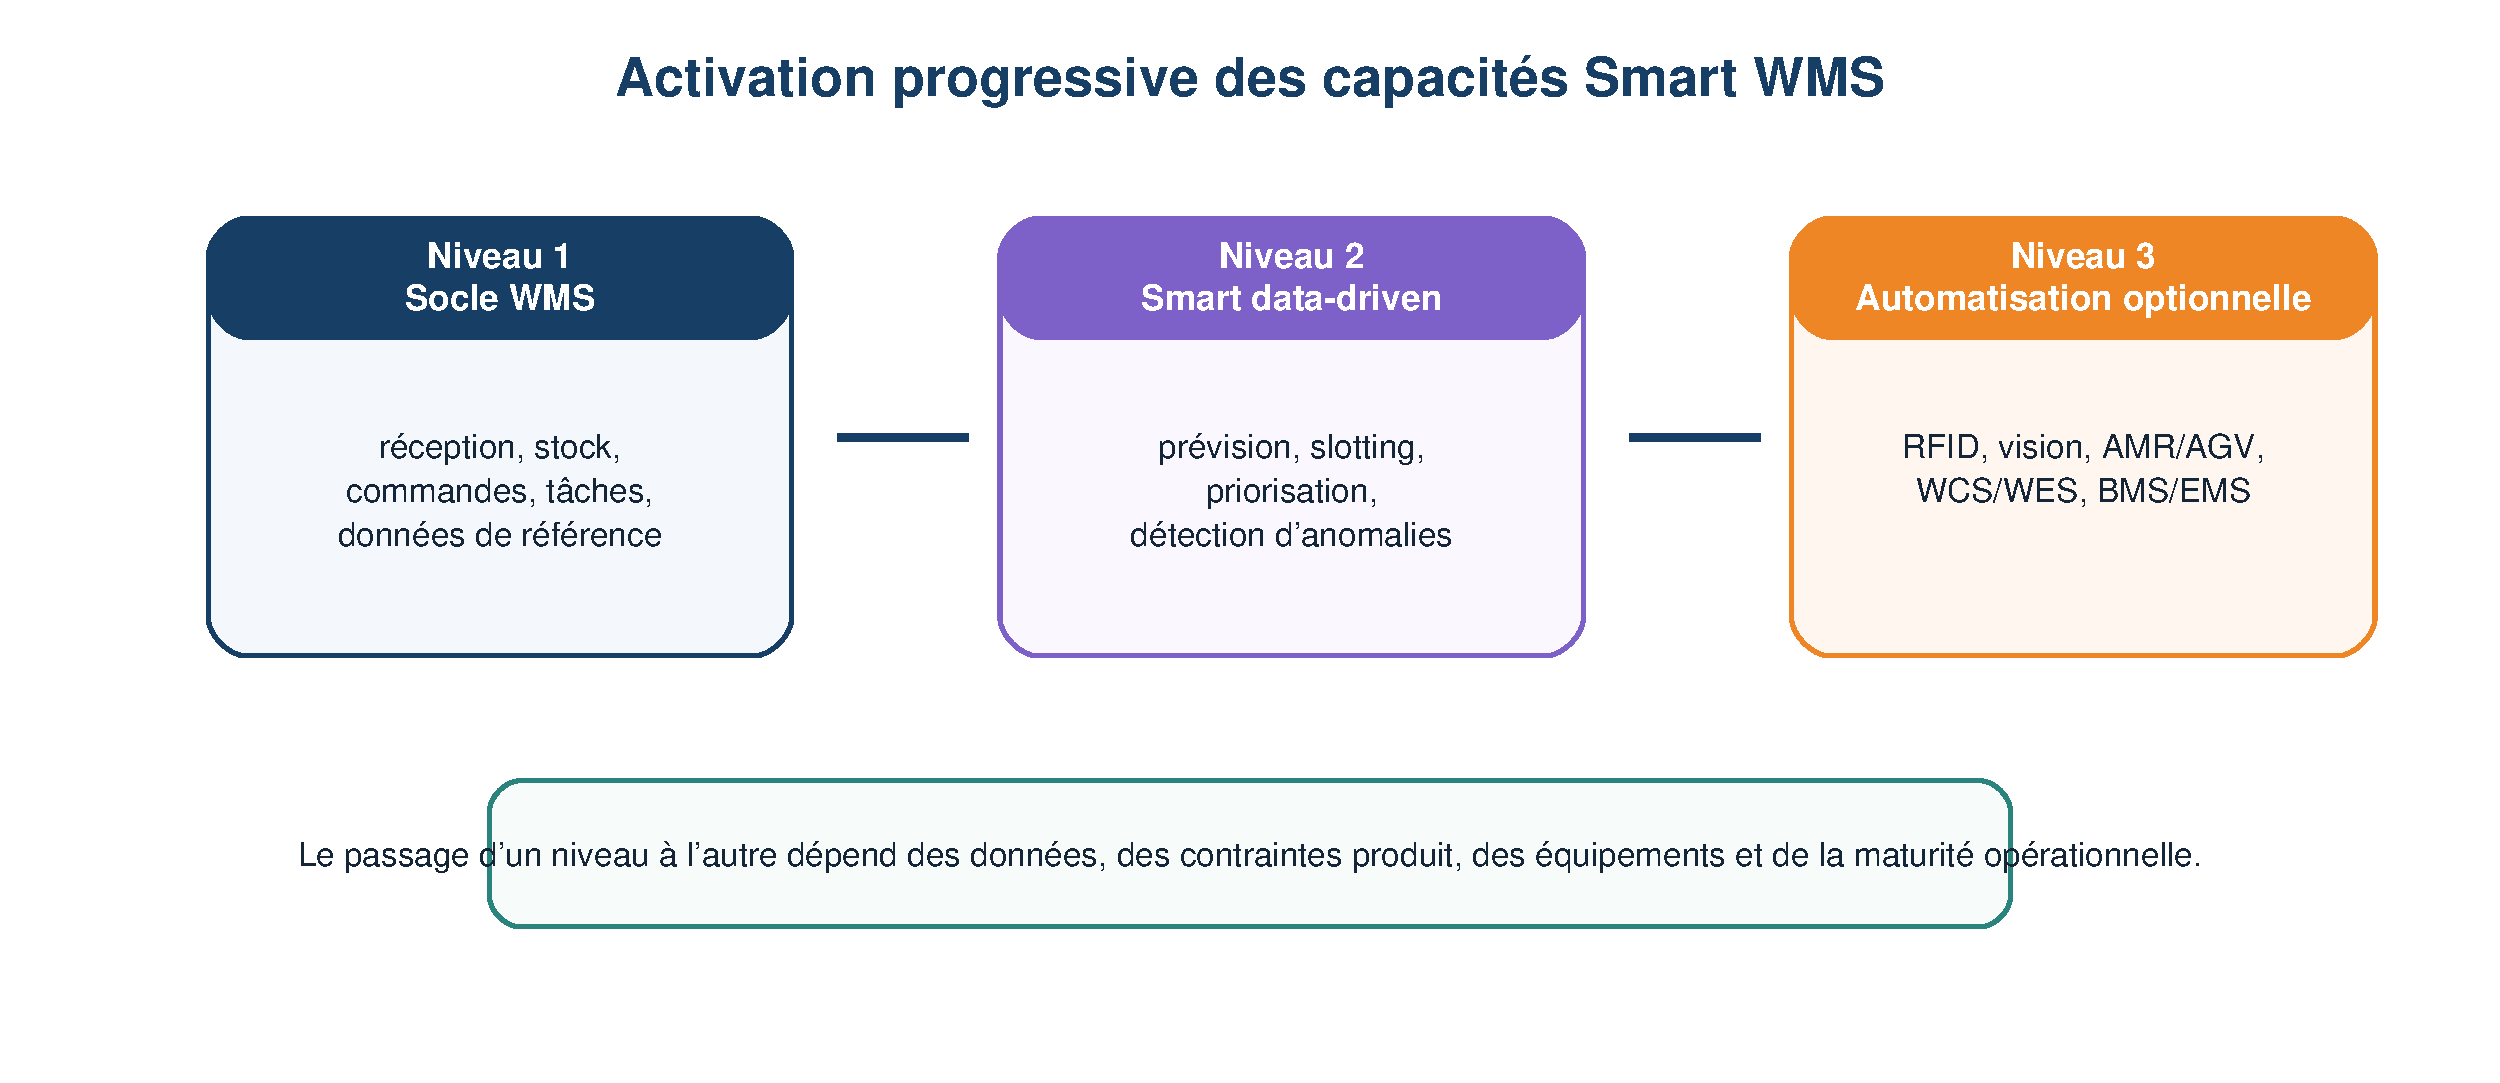
\includegraphics[width=0.92\linewidth]{figures/chapitre4/activation_progressive.pdf}
\caption{Principe d'activation progressive des capacités Smart WMS.}
\label{fig:activation-progressive}
\end{figure}

\begin{table}[H]
\centering
\caption{Responsabilités des blocs fonctionnels de l'architecture cible}
\begin{tabularx}{\linewidth}{p{3.4cm}X X}
\toprule
Bloc & Responsabilité principale & Contribution au Smart WMS \\
\midrule
Cœur opérationnel & Exécuter réception, stock, commandes, yard et expédition & Stabiliser le socle métier indispensable \\
Gestion des tâches & Créer, affecter, suivre et traiter les exceptions & Transformer décisions et alertes en actions \\
Données de référence & Structurer produits, zones, règles, rôles et unités logistiques & Donner le contexte aux règles et optimisations \\
Ressources & Gérer main-d'œuvre, équipements, actifs et interfaces & Adapter le système au niveau réel d'automatisation \\
Intelligence & Prévoir, optimiser, détecter et recommander & Améliorer la qualité des décisions opérationnelles \\
Terrain & Capturer les données et guider l'exécution & Relier le numérique au flux physique \\
\bottomrule
\end{tabularx}
\end{table}
